\section{Othello (Reversi)}

\begin{figure}[htbp]
\begin{center}
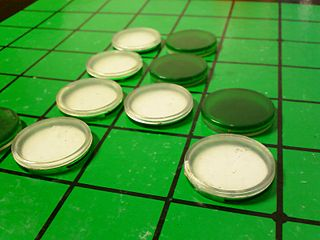
\includegraphics[width=.60\textwidth]{./imagenes/othello.jpg}
\caption{Othello}
\label{Othello}
\end{center}
\end{figure}
El reversi, Othello o Yang \footnote{\url{http://es.wikipedia.org/wiki/Othello}} es un juego entre dos personas, que comparten 64 fichas iguales, de caras distintas, que se van colocando por turnos en un tablero dividido en 64 escaques. Las caras de las fichas se distinguen por su color y cada jugador tiene asignado uno de esos colores, ganando quien tenga más fichas sobre el tablero al finalizar la partida. Se clasifica como juego de tablero, abstracto y territorial; al igual que el go y las amazonas.

La movilidad media de un jugador a lo largo de la partida es de 8 movimientos. Como en total se pueden hacer 60 movimientos, el número máximo de posibles partidas es de aproximadamente $10^{54}$. Por otra parte, el número máximo de posiciones posibles se calcula aproximadamente en $10^{30}$.

\emph{http://es.wikipedia.org/wiki/Othello 2013-05-18}

\subsubsection{¿Por qué es uno de mis juegos favoritos?}
\begin{itemize}
	\item Porque aun cuando parece un juego simple, tiene mucha profundidad. Es muy fácil de aprender, en razón de que las reglas son pocos y sencillas. Además hay versiones por todas plataformas.
\end{itemize}
